\begin{example}[Viscous Burgers 2D]
\label{ex:kucera}
Based on example in \cite[Section 1.6]{Kucera},
we will solve the equation \eqref{eq:ex_burgers} in $\Omega = [0, 1]^2$.
%\begin{equation}
%		\pdiff{u}{t} + \frac{1}{2}\left(\pdiff{u^2}{x} + \pdiff{u^2}{y}\right)  -
%		D \cdot \left( \pdiff{^2 u}{x^2} + \pdiff{^2 u}{y^2} \right)
%		= g
%\end{equation}
%where $D$ is diffusion coefficient and $g$ is a source function.
We setup the boundary condition and source function in such way that the exact
solution $u_{exact}$ is
\begin{equation}
	u_{exact} =  \ -{\left(e^{\left(-t\right)} - 1\right)} {\left(\sin\left(5 \,x
	y\right) + \sin\left(-4 \,
	x y + 4 \,x + 4 \, y\right)\right)}.
\end{equation}
We omit analytical forms of $g$ and boundary conditions for brevity.
Different values of the coefficient $C_w$ in the penalty term then yield only slightly different
convergence behavior as demonstrated in \Cref{fig:kucera_orders} and 
\ref{fig:kucera_conv}. In this case the solution does not feature any sharp steps and
an increase in the penalty coefficient leads to an increase in accuracy. In \Cref{fig:sol_kucera}
this effect is clearly visible in the numerical solution, similarly to \Cref{ex:quart1}. Kučera
in \cite{Kucera} reports average convergence rates for an irregular triangular mesh
slightly higher then ours.

\end{example}
\begin{figure}[h!]
	\centering
	\begin{tabular}{p{0.5\textwidth} p{0.5\textwidth}}
		\vspace{0pt}
		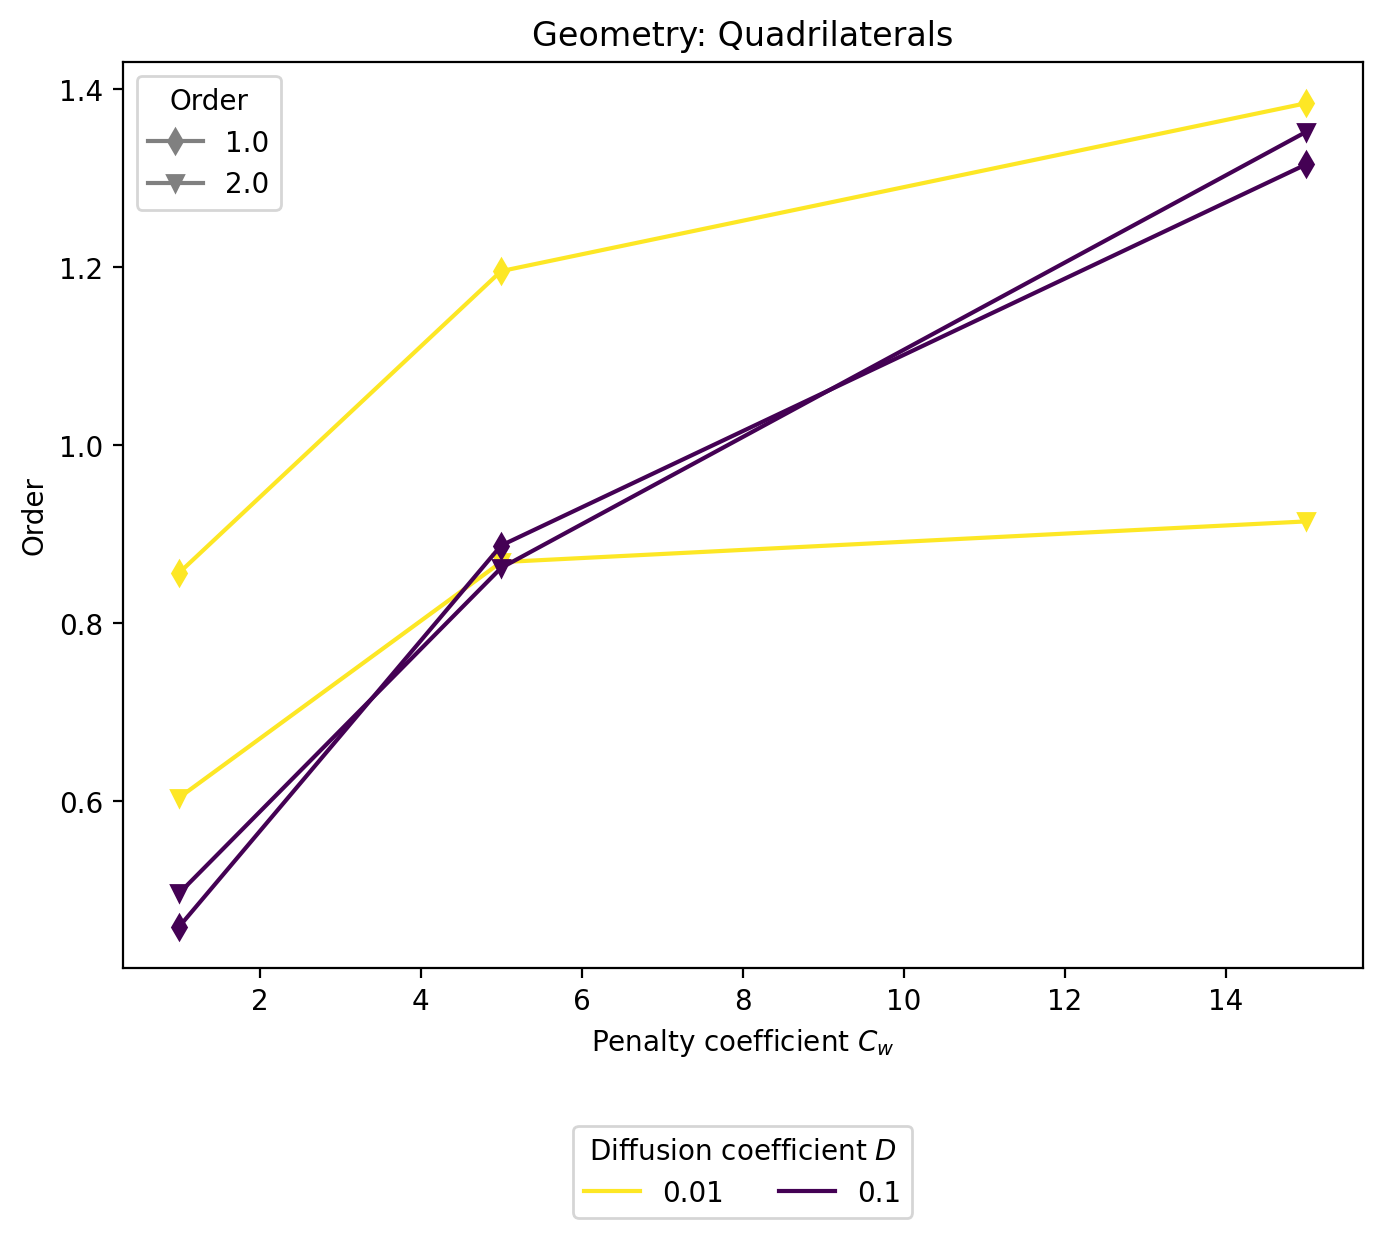
\includegraphics[width=0.49\textwidth]{../figs/parametric/burgers_2D/orders_2_4}
		&
		\vspace{0pt}
		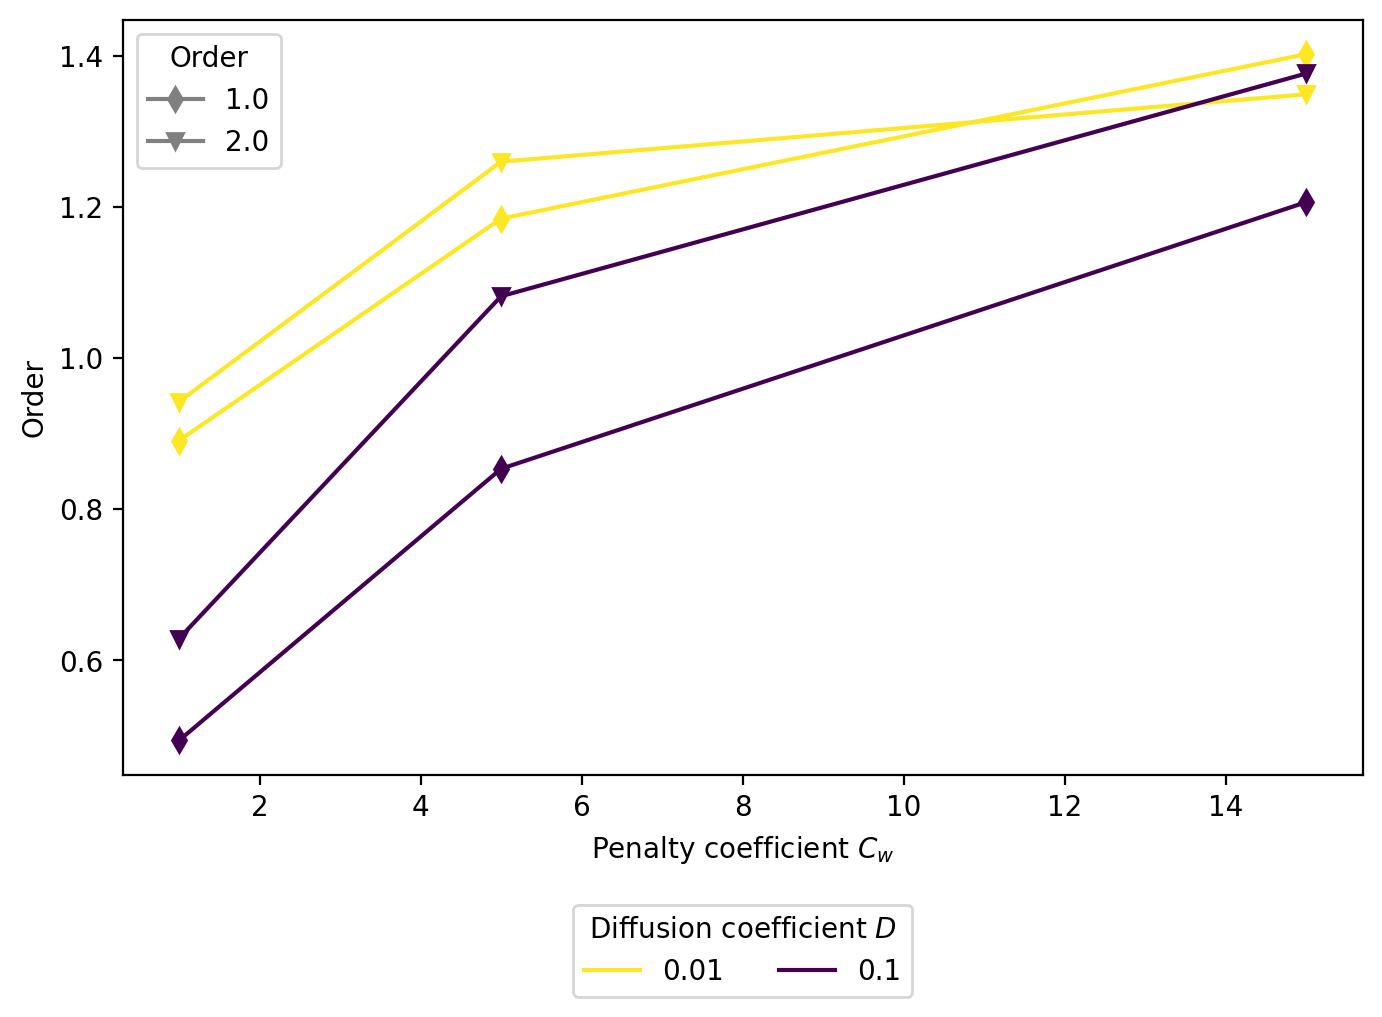
\includegraphics[width=0.49\textwidth]{../figs/parametric/burgers_2D/orders_2_3}
	\end{tabular}
	\caption{\Cref{ex:kucera}. Average orders for different values of $C_w$ for
	quadrilaterals (left) and triangles (right).}
	\label{fig:kucera_orders}
\end{figure}


\begin{figure}[h!]
	\centering
	\begin{subfigure}{.5\textwidth}
		\centering
		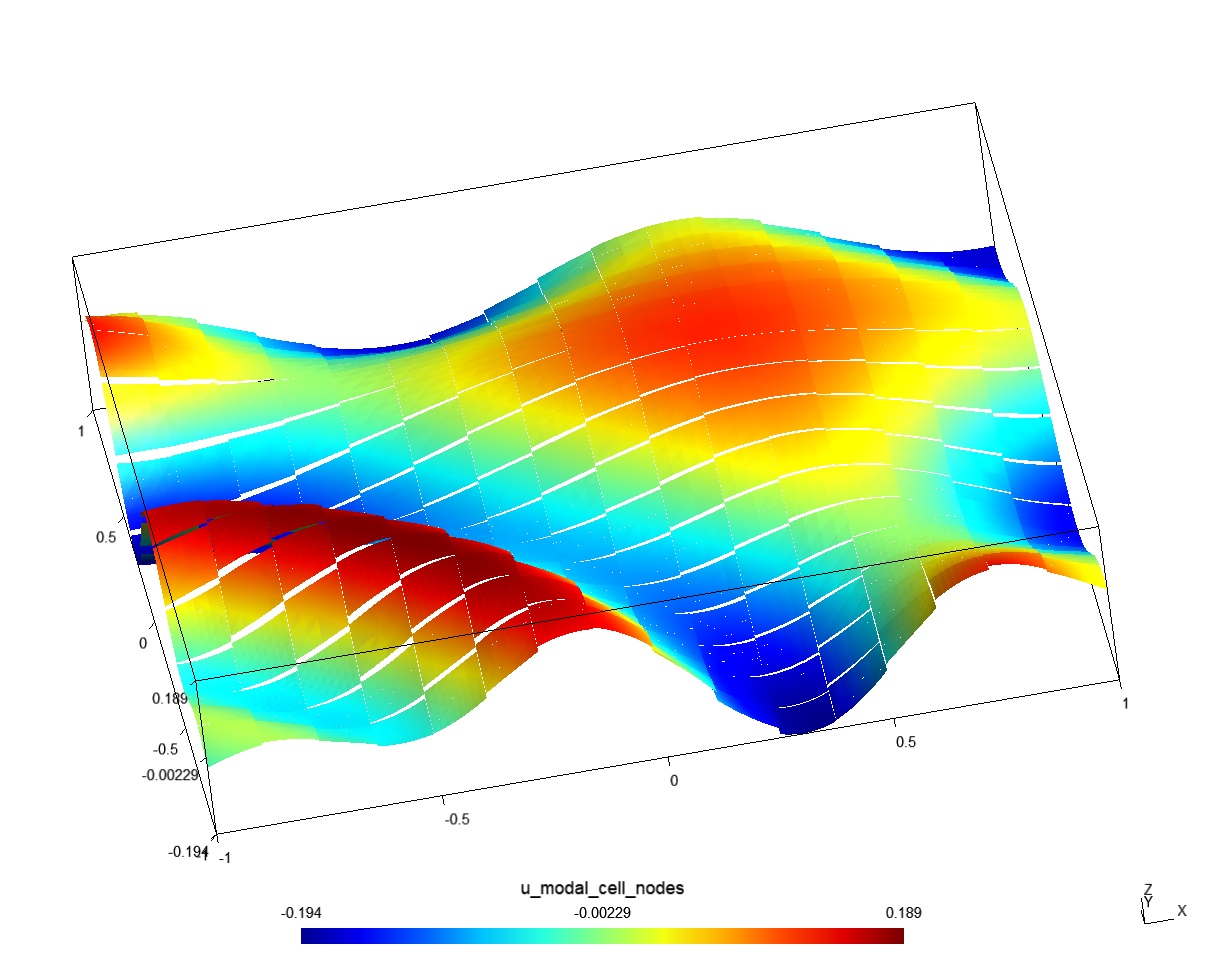
\includegraphics[width=\linewidth]{../figs/sols/kucera-010000000-sol-h256o02}
		\caption{$C_w = 1$}
	\end{subfigure}%
	\begin{subfigure}{.5\textwidth}
		\centering
		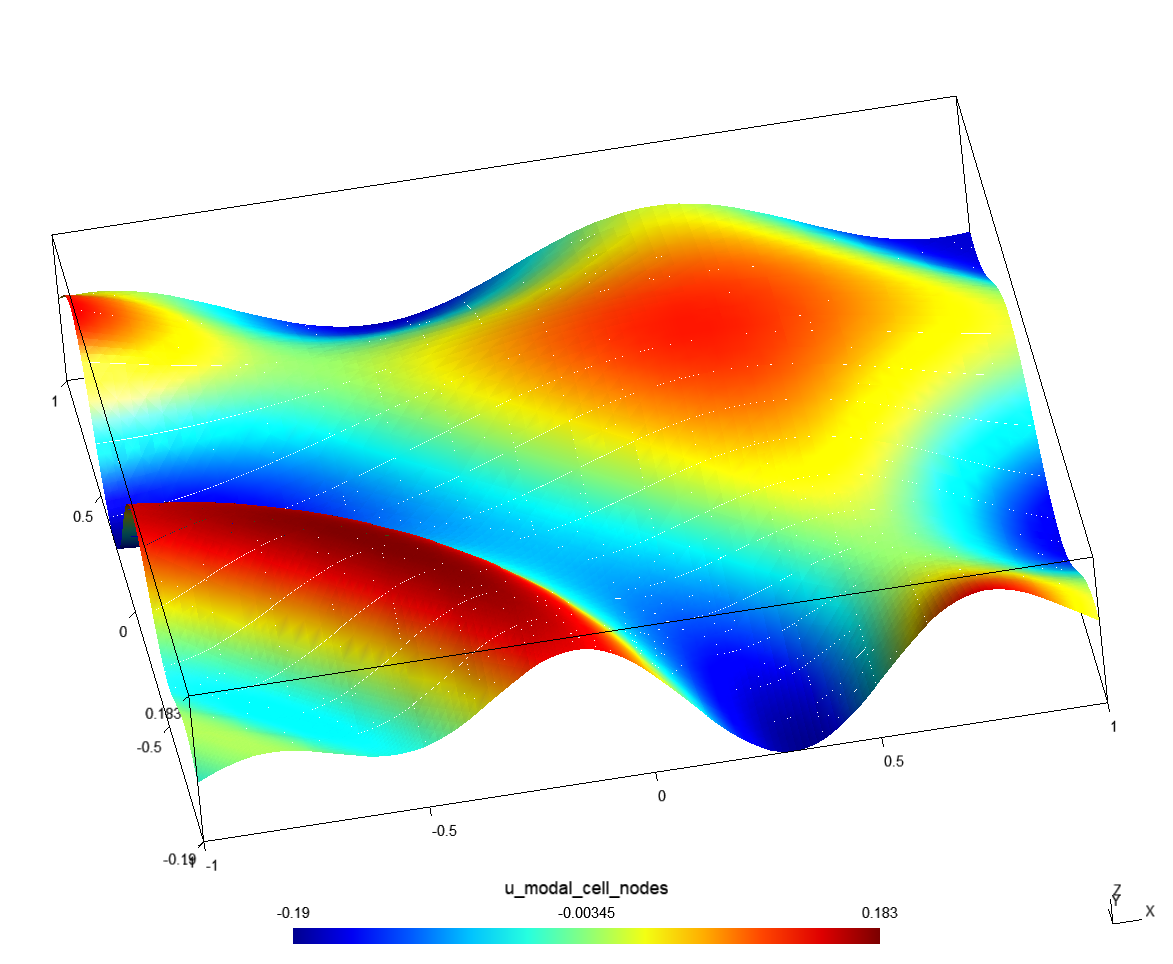
\includegraphics[width=\linewidth]{../figs/sols/kucera-212000000-sol-h256o02}
		\caption{$C_w = 15$}
	\end{subfigure}
	\caption{\Cref{ex:kucera}. Solution for different values of $C_w$ on a quadrilateral
	mesh.}
	\label{fig:sol_kucera}
\end{figure}

\begin{figure}[p!]
	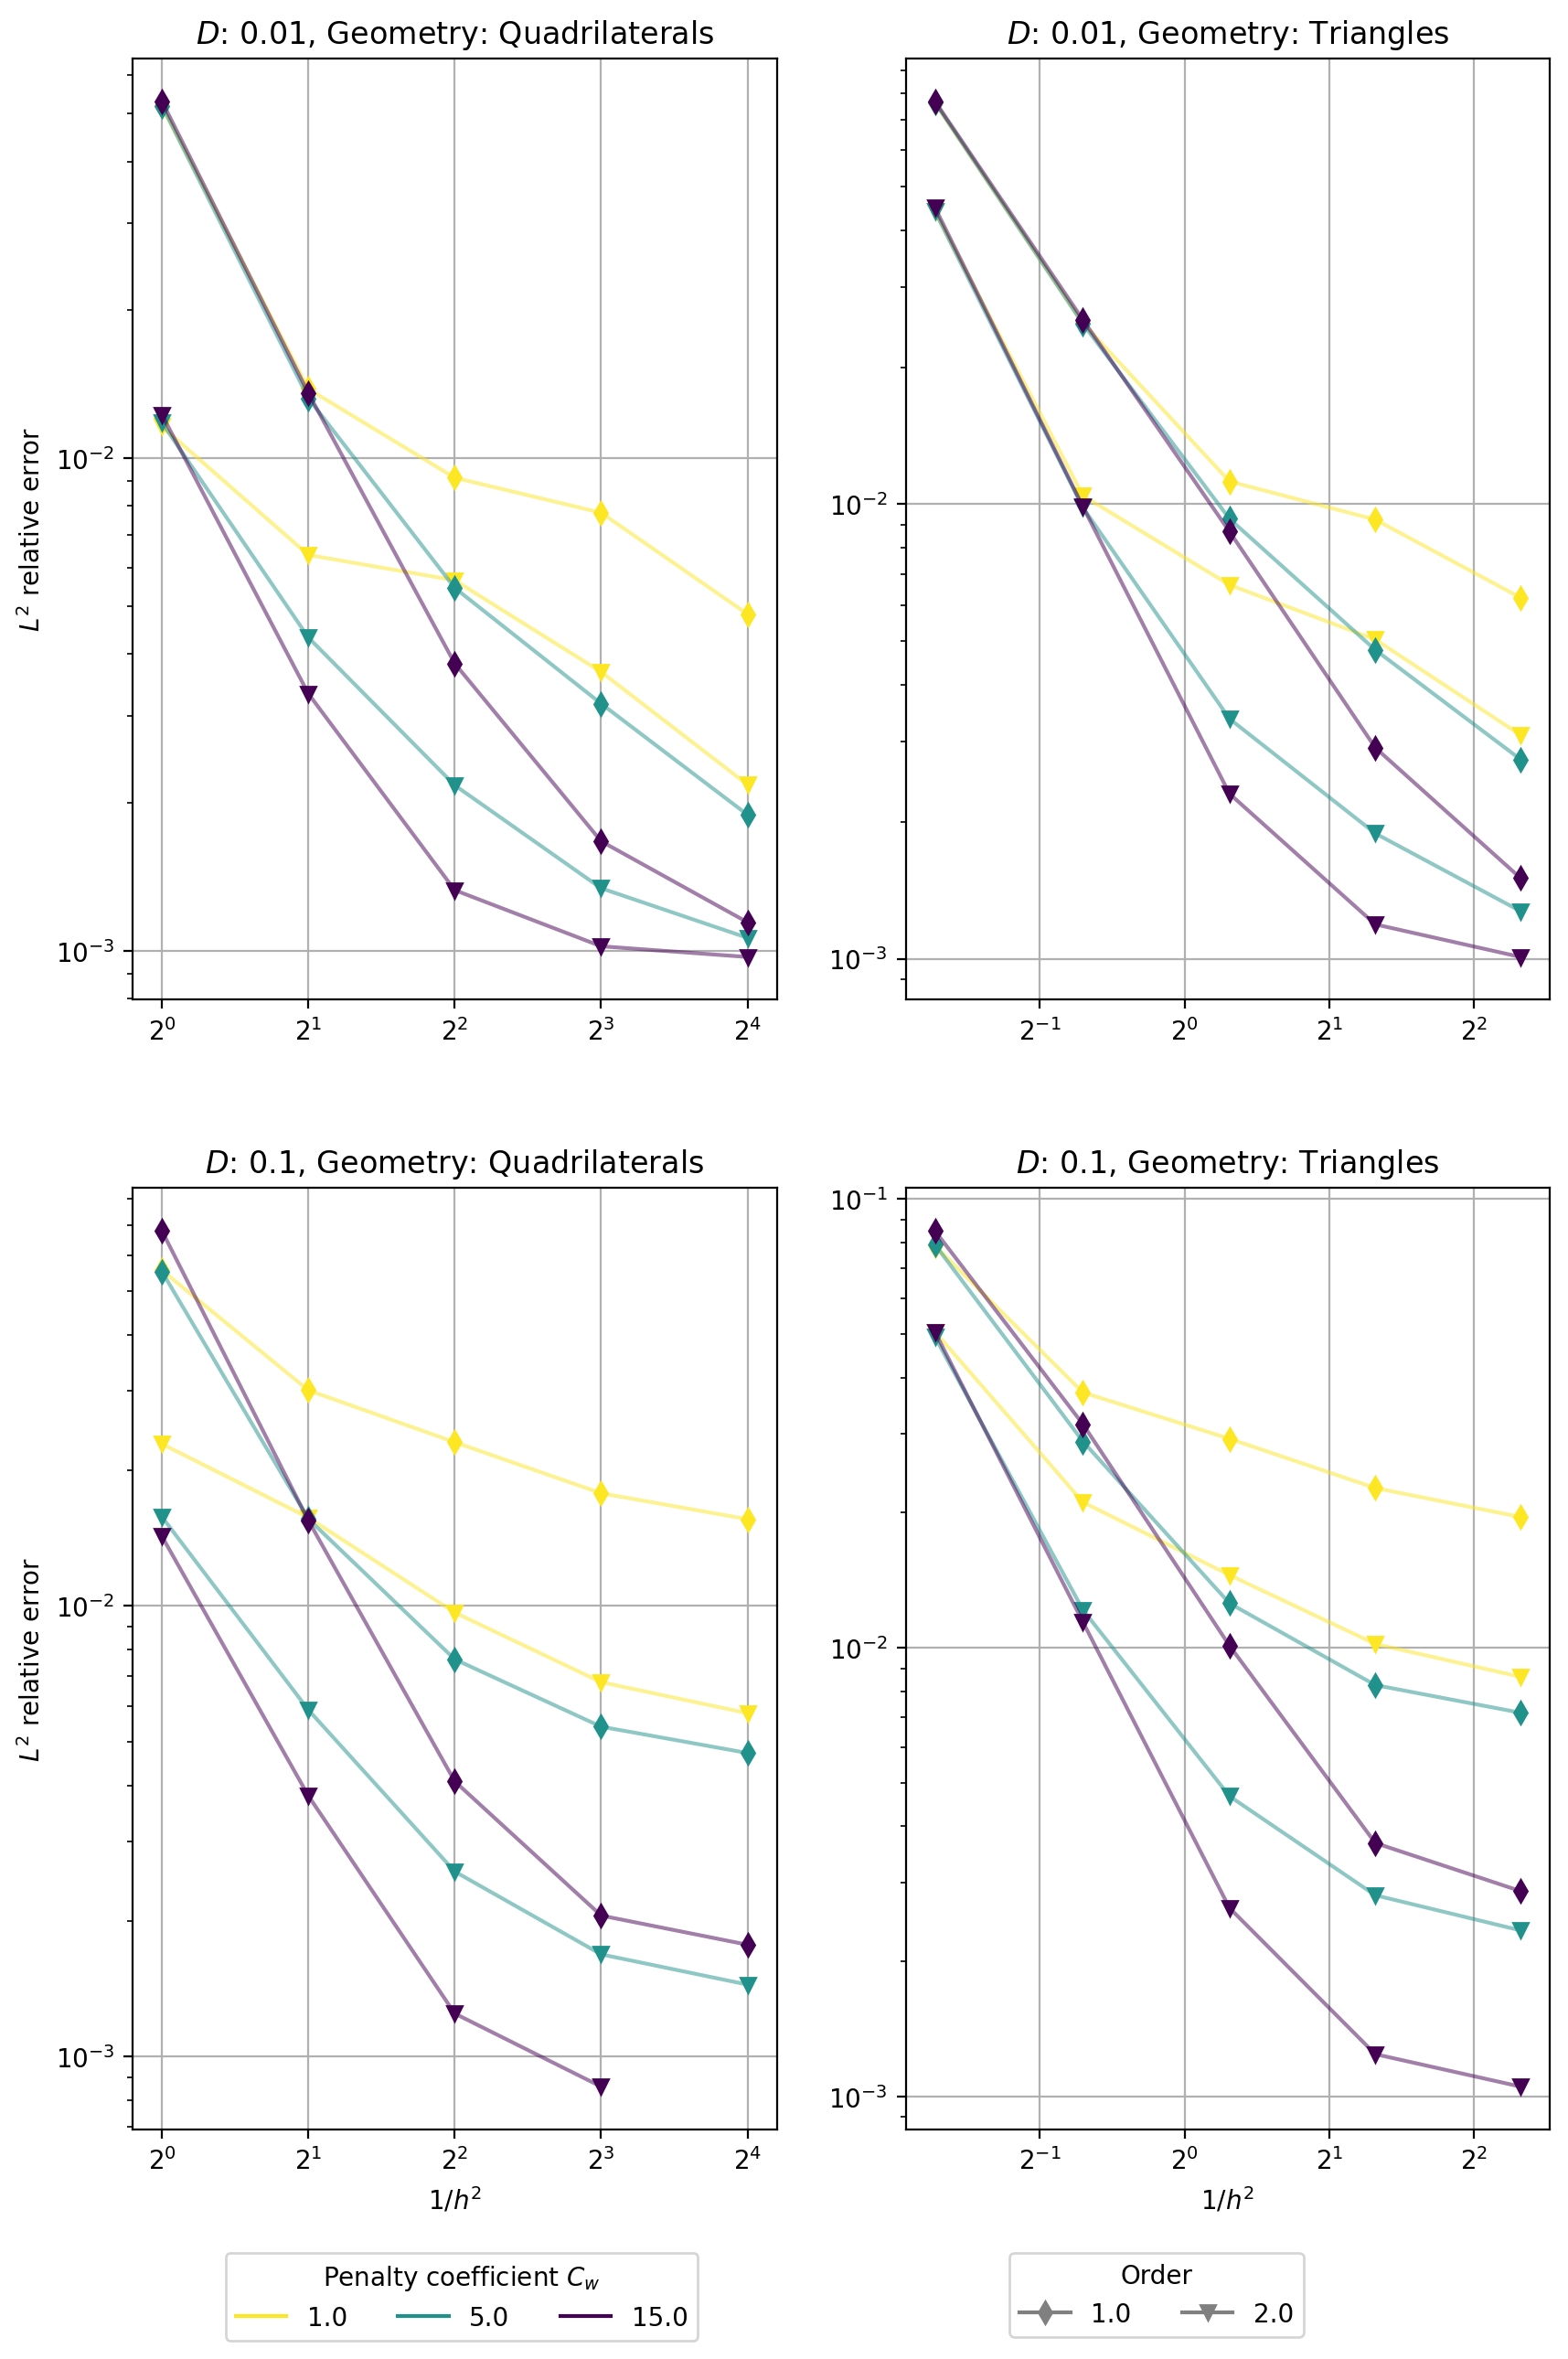
\includegraphics[width=\textwidth]{../figs/parametric/burgers_2D/convergence_symmetry}
	\caption{\Cref{ex:kucera}. Relative errors for different choices of $C_w$ for
	quadrilaterals (left) and triangles (right).}
	\label{fig:kucera_conv}
\end{figure}